\documentclass[1p]{elsarticle_modified}
%\bibliographystyle{elsarticle-num}

%\usepackage[colorlinks]{hyperref}
%\usepackage{abbrmath_seonhwa} %\Abb, \Ascr, \Acal ,\Abf, \Afrak
\usepackage{amsfonts}
\usepackage{amssymb}
\usepackage{amsmath}
\usepackage{amsthm}
\usepackage{scalefnt}
\usepackage{amsbsy}
\usepackage{kotex}
\usepackage{caption}
\usepackage{subfig}
\usepackage{color}
\usepackage{graphicx}
\usepackage{xcolor} %% white, black, red, green, blue, cyan, magenta, yellow
\usepackage{float}
\usepackage{setspace}
\usepackage{hyperref}

\usepackage{tikz}
\usetikzlibrary{arrows}

\usepackage{multirow}
\usepackage{array} % fixed length table
\usepackage{hhline}

%%%%%%%%%%%%%%%%%%%%%
\makeatletter
\renewcommand*\env@matrix[1][\arraystretch]{%
	\edef\arraystretch{#1}%
	\hskip -\arraycolsep
	\let\@ifnextchar\new@ifnextchar
	\array{*\c@MaxMatrixCols c}}
\makeatother %https://tex.stackexchange.com/questions/14071/how-can-i-increase-the-line-spacing-in-a-matrix
%%%%%%%%%%%%%%%

\usepackage[normalem]{ulem}

\newcommand{\msout}[1]{\ifmmode\text{\sout{\ensuremath{#1}}}\else\sout{#1}\fi}
%SOURCE: \msout is \stkout macro in https://tex.stackexchange.com/questions/20609/strikeout-in-math-mode

\newcommand{\cancel}[1]{
	\ifmmode
	{\color{red}\msout{#1}}
	\else
	{\color{red}\sout{#1}}
	\fi
}

\newcommand{\add}[1]{
	{\color{blue}\uwave{#1}}
}

\newcommand{\replace}[2]{
	\ifmmode
	{\color{red}\msout{#1}}{\color{blue}\uwave{#2}}
	\else
	{\color{red}\sout{#1}}{\color{blue}\uwave{#2}}
	\fi
}

\newcommand{\Sol}{\mathcal{S}} %segment
\newcommand{\D}{D} %diagram
\newcommand{\A}{\mathcal{A}} %arc


%%%%%%%%%%%%%%%%%%%%%%%%%%%%%5 test

\def\sl{\operatorname{\textup{SL}}(2,\Cbb)}
\def\psl{\operatorname{\textup{PSL}}(2,\Cbb)}
\def\quan{\mkern 1mu \triangleright \mkern 1mu}

\theoremstyle{definition}
\newtheorem{thm}{Theorem}[section]
\newtheorem{prop}[thm]{Proposition}
\newtheorem{lem}[thm]{Lemma}
\newtheorem{ques}[thm]{Question}
\newtheorem{cor}[thm]{Corollary}
\newtheorem{defn}[thm]{Definition}
\newtheorem{exam}[thm]{Example}
\newtheorem{rmk}[thm]{Remark}
\newtheorem{alg}[thm]{Algorithm}

\newcommand{\I}{\sqrt{-1}}
\begin{document}

%\begin{frontmatter}
%
%\title{Boundary parabolic representations of knots up to 8 crossings}
%
%%% Group authors per affiliation:
%\author{Yunhi Cho} 
%\address{Department of Mathematics, University of Seoul, Seoul, Korea}
%\ead{yhcho@uos.ac.kr}
%
%
%\author{Seonhwa Kim} %\fnref{s_kim}}
%\address{Center for Geometry and Physics, Institute for Basic Science, Pohang, 37673, Korea}
%\ead{ryeona17@ibs.re.kr}
%
%\author{Hyuk Kim}
%\address{Department of Mathematical Sciences, Seoul National University, Seoul 08826, Korea}
%\ead{hyukkim@snu.ac.kr}
%
%\author{Seokbeom Yoon}
%\address{Department of Mathematical Sciences, Seoul National University, Seoul, 08826,  Korea}
%\ead{sbyoon15@snu.ac.kr}
%
%\begin{abstract}
%We find all boundary parabolic representation of knots up to 8 crossings.
%
%\end{abstract}
%\begin{keyword}
%    \MSC[2010] 57M25 
%\end{keyword}
%
%\end{frontmatter}

%\linenumbers
%\tableofcontents
%
\newcommand\colored[1]{\textcolor{white}{\rule[-0.35ex]{0.8em}{1.4ex}}\kern-0.8em\color{red} #1}%
%\newcommand\colored[1]{\textcolor{white}{ #1}\kern-2.17ex	\textcolor{white}{ #1}\kern-1.81ex	\textcolor{white}{ #1}\kern-2.15ex\color{red}#1	}

{\Large $\underline{11n_{91}~(K11n_{91})}$}

\setlength{\tabcolsep}{10pt}
\renewcommand{\arraystretch}{1.6}
\vspace{1cm}\begin{tabular}{m{100pt}>{\centering\arraybackslash}m{274pt}}
\multirow{5}{120pt}{
	\centering
	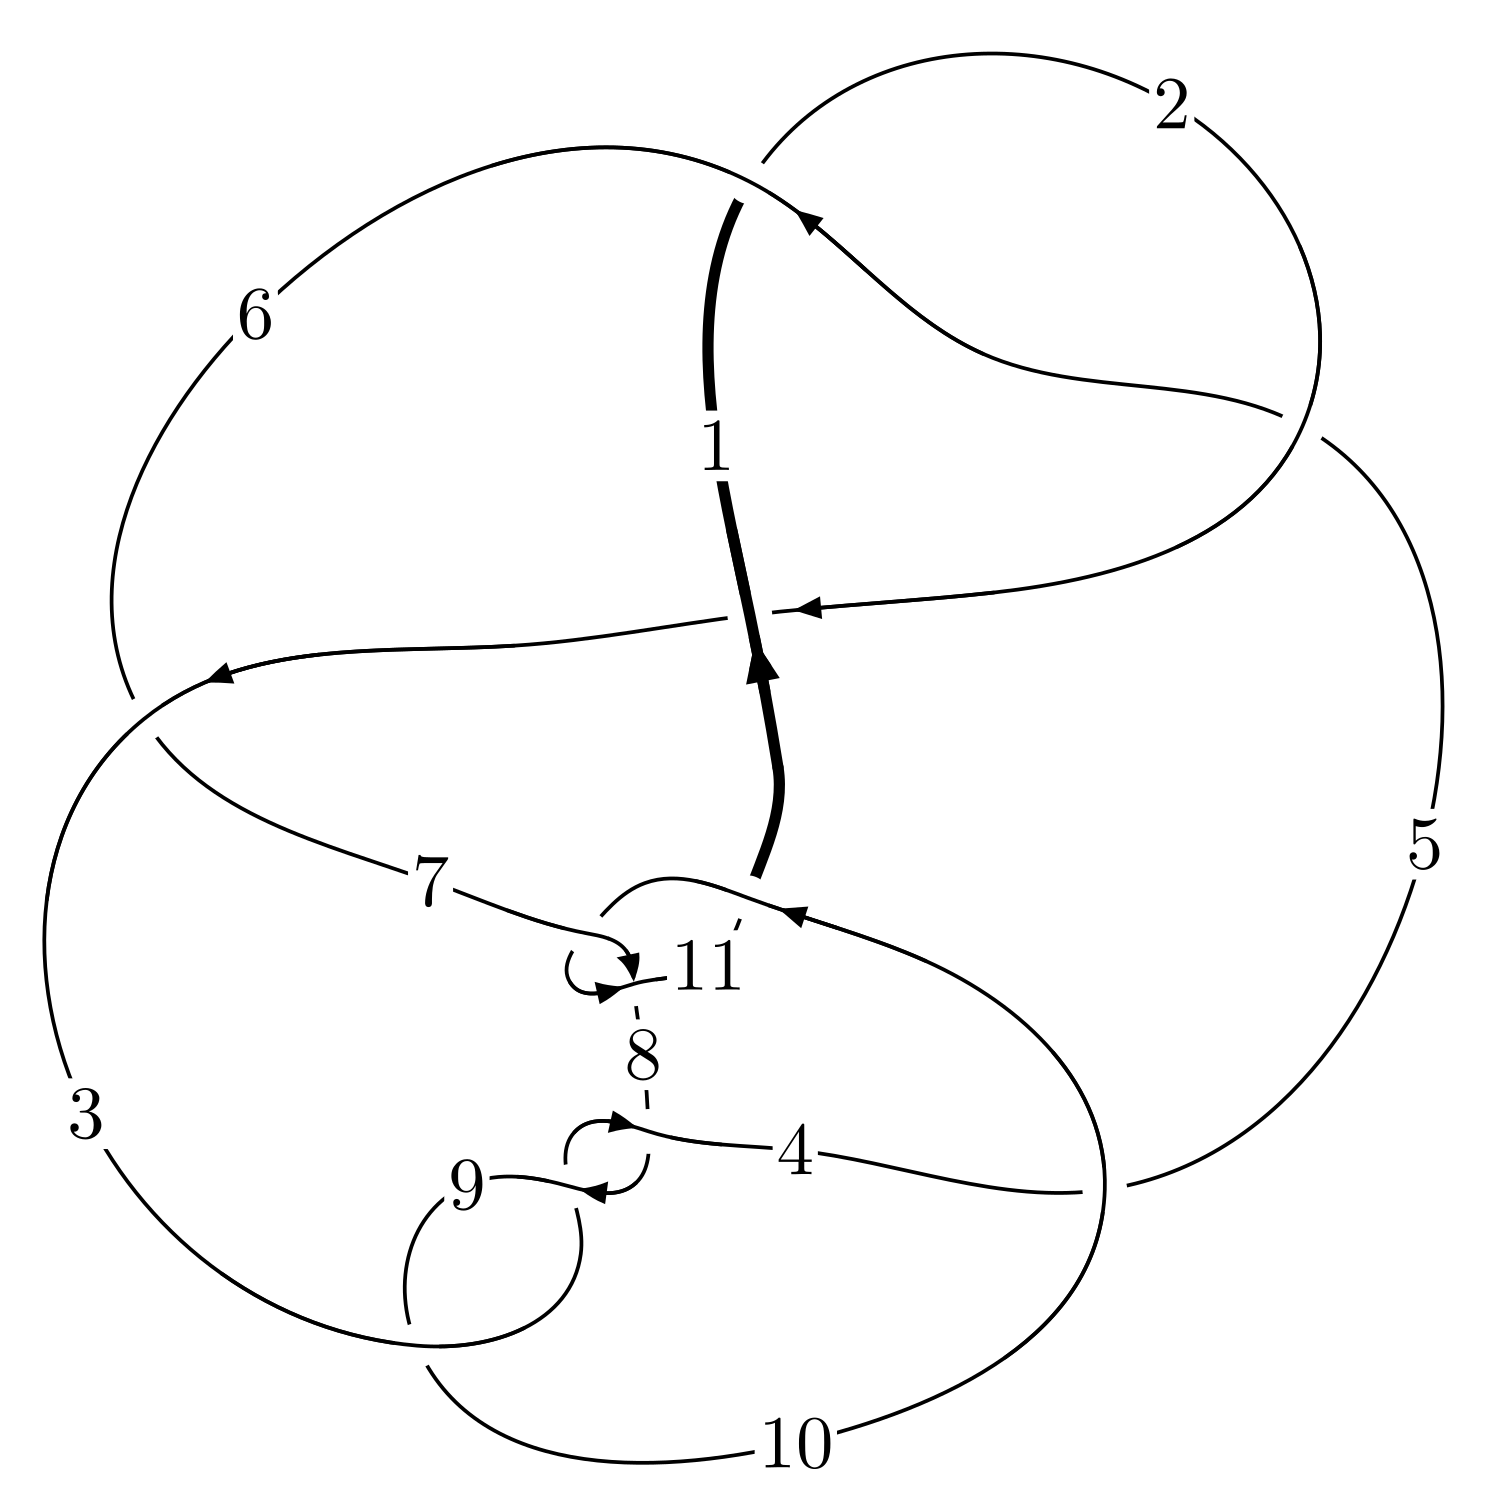
\includegraphics[width=112pt]{../../../GIT/diagram.site/Diagrams/png/707_11n_91.png}\\
\ \ \ A knot diagram\footnotemark}&
\allowdisplaybreaks
\textbf{Linearized knot diagam} \\
\cline{2-2}
 &
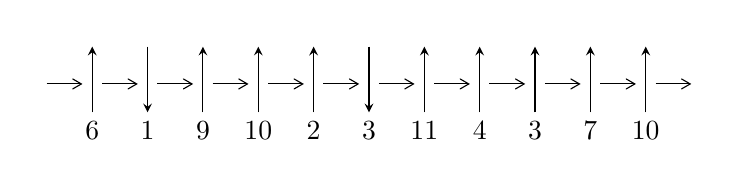
\begin{tikzpicture}[x=20pt, y=17pt]
	% nodes
	\node (C0) at (0, 0) {};
	\node (C1) at (1, 0) {};
	\node (C1U) at (1, +1) {};
	\node (C1D) at (1, -1) {6};

	\node (C2) at (2, 0) {};
	\node (C2U) at (2, +1) {};
	\node (C2D) at (2, -1) {1};

	\node (C3) at (3, 0) {};
	\node (C3U) at (3, +1) {};
	\node (C3D) at (3, -1) {9};

	\node (C4) at (4, 0) {};
	\node (C4U) at (4, +1) {};
	\node (C4D) at (4, -1) {10};

	\node (C5) at (5, 0) {};
	\node (C5U) at (5, +1) {};
	\node (C5D) at (5, -1) {2};

	\node (C6) at (6, 0) {};
	\node (C6U) at (6, +1) {};
	\node (C6D) at (6, -1) {3};

	\node (C7) at (7, 0) {};
	\node (C7U) at (7, +1) {};
	\node (C7D) at (7, -1) {11};

	\node (C8) at (8, 0) {};
	\node (C8U) at (8, +1) {};
	\node (C8D) at (8, -1) {4};

	\node (C9) at (9, 0) {};
	\node (C9U) at (9, +1) {};
	\node (C9D) at (9, -1) {3};

	\node (C10) at (10, 0) {};
	\node (C10U) at (10, +1) {};
	\node (C10D) at (10, -1) {7};

	\node (C11) at (11, 0) {};
	\node (C11U) at (11, +1) {};
	\node (C11D) at (11, -1) {10};
	\node (C12) at (12, 0) {};

	% arrows
	\draw[->,>={angle 60}]
	(C0) edge (C1) (C1) edge (C2) (C2) edge (C3) (C3) edge (C4) (C4) edge (C5) (C5) edge (C6) (C6) edge (C7) (C7) edge (C8) (C8) edge (C9) (C9) edge (C10) (C10) edge (C11) (C11) edge (C12) ;	\draw[->,>=stealth]
	(C1D) edge (C1U) (C2U) edge (C2D) (C3D) edge (C3U) (C4D) edge (C4U) (C5D) edge (C5U) (C6U) edge (C6D) (C7D) edge (C7U) (C8D) edge (C8U) (C9D) edge (C9U) (C10D) edge (C10U) (C11D) edge (C11U) ;
	\end{tikzpicture} \\
\hhline{~~} \\& 
\textbf{Solving Sequence} \\ \cline{2-2} 
 &
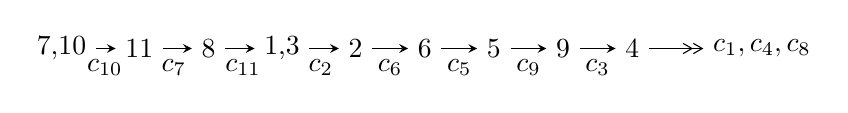
\begin{tikzpicture}[x=25pt, y=7pt]
	% node
	\node (A0) at (-1/8, 0) {7,10};
	\node (A1) at (1, 0) {11};
	\node (A2) at (2, 0) {8};
	\node (A3) at (49/16, 0) {1,3};
	\node (A4) at (33/8, 0) {2};
	\node (A5) at (41/8, 0) {6};
	\node (A6) at (49/8, 0) {5};
	\node (A7) at (57/8, 0) {9};
	\node (A8) at (65/8, 0) {4};
	\node (C1) at (1/2, -1) {$c_{10}$};
	\node (C2) at (3/2, -1) {$c_{7}$};
	\node (C3) at (5/2, -1) {$c_{11}$};
	\node (C4) at (29/8, -1) {$c_{2}$};
	\node (C5) at (37/8, -1) {$c_{6}$};
	\node (C6) at (45/8, -1) {$c_{5}$};
	\node (C7) at (53/8, -1) {$c_{9}$};
	\node (C8) at (61/8, -1) {$c_{3}$};
	\node (A9) at (10, 0) {$c_{1},c_{4},c_{8}$};

	% edge
	\draw[->,>=stealth]	
	(A0) edge (A1) (A1) edge (A2) (A2) edge (A3) (A3) edge (A4) (A4) edge (A5) (A5) edge (A6) (A6) edge (A7) (A7) edge (A8) ;
	\draw[->>,>={angle 60}]	
	(A8) edge (A9);
\end{tikzpicture} \\ 

\end{tabular} \\

\footnotetext{
The image of knot diagram is generated by the software ``\textbf{Draw programme}" developed by Andrew Bartholomew(\url{http://www.layer8.co.uk/maths/draw/index.htm\#Running-draw}), where we modified some parts for our purpose(\url{https://github.com/CATsTAILs/LinksPainter}).
}\phantom \\ \newline 
\centering \textbf{Ideals for irreducible components\footnotemark of $X_{\text{par}}$} 
 
\begin{align*}
I^u_{1}&=\langle 
-10091257321 u^{20}+17716980292 u^{19}+\cdots+366196956382 b+49796914345,\\
\phantom{I^u_{1}}&\phantom{= \langle  }591910942537 u^{20}-2794488596145 u^{19}+\cdots+4394363476584 a-481484753828,\\
\phantom{I^u_{1}}&\phantom{= \langle  }u^{21}-3 u^{20}+\cdots-2 u-3\rangle \\
I^u_{2}&=\langle 
b^2+2,\;a^2- a+1,\;u+1\rangle \\
I^u_{3}&=\langle 
b,\;a^2- a+1,\;u-1\rangle \\
\\
\end{align*}
\raggedright * 3 irreducible components of $\dim_{\mathbb{C}}=0$, with total 27 representations.\\
\footnotetext{All coefficients of polynomials are rational numbers. But the coefficients are sometimes approximated in decimal forms when there is not enough margin.}
\newpage
\renewcommand{\arraystretch}{1}
\centering \section*{I. $I^u_{1}= \langle -1.01\times10^{10} u^{20}+1.77\times10^{10} u^{19}+\cdots+3.66\times10^{11} b+4.98\times10^{10},\;5.92\times10^{11} u^{20}-2.79\times10^{12} u^{19}+\cdots+4.39\times10^{12} a-4.81\times10^{11},\;u^{21}-3 u^{20}+\cdots-2 u-3 \rangle$}
\flushleft \textbf{(i) Arc colorings}\\
\begin{tabular}{m{7pt} m{180pt} m{7pt} m{180pt} }
\flushright $a_{7}=$&$\begin{pmatrix}0\\u\end{pmatrix}$ \\
\flushright $a_{10}=$&$\begin{pmatrix}1\\0\end{pmatrix}$ \\
\flushright $a_{11}=$&$\begin{pmatrix}1\\- u^2\end{pmatrix}$ \\
\flushright $a_{8}=$&$\begin{pmatrix}u\\- u^3+u\end{pmatrix}$ \\
\flushright $a_{1}=$&$\begin{pmatrix}- u^2+1\\- u^2\end{pmatrix}$ \\
\flushright $a_{3}=$&$\begin{pmatrix}-0.134698 u^{20}+0.635926 u^{19}+\cdots-0.0316545 u+0.109569\\0.0275569 u^{20}-0.0483810 u^{19}+\cdots-1.11621 u-0.135984\end{pmatrix}$ \\
\flushright $a_{2}=$&$\begin{pmatrix}-0.0599090 u^{20}+0.413165 u^{19}+\cdots-1.26842 u+0.402548\\0.129090 u^{20}-0.405931 u^{19}+\cdots-1.14509 u-0.299649\end{pmatrix}$ \\
\flushright $a_{6}=$&$\begin{pmatrix}-0.0944207 u^{20}+0.398371 u^{19}+\cdots+0.793023 u-0.448119\\0.0612997 u^{20}-0.138407 u^{19}+\cdots+0.143901 u-0.565085\end{pmatrix}$ \\
\flushright $a_{5}=$&$\begin{pmatrix}0.340816 u^{20}-1.13692 u^{19}+\cdots-0.307450 u-1.55518\\0.154312 u^{20}-0.484554 u^{19}+\cdots-0.533633 u-0.125533\end{pmatrix}$ \\
\flushright $a_{9}=$&$\begin{pmatrix}-0.188362 u^{20}+0.626385 u^{19}+\cdots+2.11578 u+0.520624\\0.0158081 u^{20}+0.0256218 u^{19}+\cdots+0.586386 u-0.748984\end{pmatrix}$ \\
\flushright $a_{4}=$&$\begin{pmatrix}-0.186504 u^{20}+0.652367 u^{19}+\cdots-0.226183 u+1.42965\\-0.154312 u^{20}+0.484554 u^{19}+\cdots+0.533633 u+0.125533\end{pmatrix}$\\ \flushright $a_{4}=$&$\begin{pmatrix}-0.186504 u^{20}+0.652367 u^{19}+\cdots-0.226183 u+1.42965\\-0.154312 u^{20}+0.484554 u^{19}+\cdots+0.533633 u+0.125533\end{pmatrix}$\\&\end{tabular}
\flushleft \textbf{(ii) Obstruction class $= -1$}\\~\\
\flushleft \textbf{(iii) Cusp Shapes $= \frac{57646172449}{732393912764} u^{20}+\frac{387941164973}{732393912764} u^{19}+\cdots+\frac{4279700760483}{732393912764} u+\frac{1134852296901}{183098478191}$}\\~\\
\newpage\renewcommand{\arraystretch}{1}
\flushleft \textbf{(iv) u-Polynomials at the component}\newline \\
\begin{tabular}{m{50pt}|m{274pt}}
Crossings & \hspace{64pt}u-Polynomials at each crossing \\
\hline $$\begin{aligned}c_{1},c_{5}\end{aligned}$$&$\begin{aligned}
&u^{21}-2 u^{20}+\cdots+7 u-3
\end{aligned}$\\
\hline $$\begin{aligned}c_{2}\end{aligned}$$&$\begin{aligned}
&u^{21}+14 u^{20}+\cdots+49 u-9
\end{aligned}$\\
\hline $$\begin{aligned}c_{3},c_{8},c_{9}\end{aligned}$$&$\begin{aligned}
&u^{21}+u^{20}+\cdots+8 u-4
\end{aligned}$\\
\hline $$\begin{aligned}c_{4}\end{aligned}$$&$\begin{aligned}
&u^{21}- u^{20}+\cdots-64 u-548
\end{aligned}$\\
\hline $$\begin{aligned}c_{6}\end{aligned}$$&$\begin{aligned}
&u^{21}+2 u^{20}+\cdots+19 u-3
\end{aligned}$\\
\hline $$\begin{aligned}c_{7},c_{10}\end{aligned}$$&$\begin{aligned}
&u^{21}-3 u^{20}+\cdots-2 u-3
\end{aligned}$\\
\hline $$\begin{aligned}c_{11}\end{aligned}$$&$\begin{aligned}
&u^{21}-3 u^{20}+\cdots+22 u-9
\end{aligned}$\\
\hline
\end{tabular}\\~\\
\newpage\renewcommand{\arraystretch}{1}
\flushleft \textbf{(v) Riley Polynomials at the component}\newline \\
\begin{tabular}{m{50pt}|m{274pt}}
Crossings & \hspace{64pt}Riley Polynomials at each crossing \\
\hline $$\begin{aligned}c_{1},c_{5}\end{aligned}$$&$\begin{aligned}
&y^{21}+14 y^{20}+\cdots+49 y-9
\end{aligned}$\\
\hline $$\begin{aligned}c_{2}\end{aligned}$$&$\begin{aligned}
&y^{21}-10 y^{20}+\cdots+7117 y-81
\end{aligned}$\\
\hline $$\begin{aligned}c_{3},c_{8},c_{9}\end{aligned}$$&$\begin{aligned}
&y^{21}+31 y^{20}+\cdots-160 y-16
\end{aligned}$\\
\hline $$\begin{aligned}c_{4}\end{aligned}$$&$\begin{aligned}
&y^{21}+91 y^{20}+\cdots-4121248 y-300304
\end{aligned}$\\
\hline $$\begin{aligned}c_{6}\end{aligned}$$&$\begin{aligned}
&y^{21}-34 y^{20}+\cdots+193 y-9
\end{aligned}$\\
\hline $$\begin{aligned}c_{7},c_{10}\end{aligned}$$&$\begin{aligned}
&y^{21}-3 y^{20}+\cdots+22 y-9
\end{aligned}$\\
\hline $$\begin{aligned}c_{11}\end{aligned}$$&$\begin{aligned}
&y^{21}+37 y^{20}+\cdots+2158 y-81
\end{aligned}$\\
\hline
\end{tabular}\\~\\
\newpage\flushleft \textbf{(vi) Complex Volumes and Cusp Shapes}
$$\begin{array}{c|c|c}  
\text{Solutions to }I^u_{1}& \I (\text{vol} + \sqrt{-1}CS) & \text{Cusp shape}\\
 \hline 
\begin{aligned}
u &= -0.678453 + 0.688147 I \\
a &= \phantom{-}0.845365 + 0.796760 I \\
b &= -0.271568 + 1.062540 I\end{aligned}
 & -2.57223 - 2.30104 I & \phantom{-}5.12347 + 3.68698 I \\ \hline\begin{aligned}
u &= -0.678453 - 0.688147 I \\
a &= \phantom{-}0.845365 - 0.796760 I \\
b &= -0.271568 - 1.062540 I\end{aligned}
 & -2.57223 + 2.30104 I & \phantom{-}5.12347 - 3.68698 I \\ \hline\begin{aligned}
u &= \phantom{-}0.316999 + 0.813917 I \\
a &= -0.403688 + 0.492380 I \\
b &= \phantom{-}0.713808 + 0.270061 I\end{aligned}
 & -2.21076 + 2.09468 I & \phantom{-}3.00496 - 3.91489 I \\ \hline\begin{aligned}
u &= \phantom{-}0.316999 - 0.813917 I \\
a &= -0.403688 - 0.492380 I \\
b &= \phantom{-}0.713808 - 0.270061 I\end{aligned}
 & -2.21076 - 2.09468 I & \phantom{-}3.00496 + 3.91489 I \\ \hline\begin{aligned}
u &= \phantom{-}1.145710 + 0.140166 I \\
a &= \phantom{-}0.239466 - 0.410115 I \\
b &= -0.264392 + 0.442489 I\end{aligned}
 & \phantom{-}1.11524 + 1.37460 I & \phantom{-}4.04933 + 2.02582 I \\ \hline\begin{aligned}
u &= \phantom{-}1.145710 - 0.140166 I \\
a &= \phantom{-}0.239466 + 0.410115 I \\
b &= -0.264392 - 0.442489 I\end{aligned}
 & \phantom{-}1.11524 - 1.37460 I & \phantom{-}4.04933 - 2.02582 I \\ \hline\begin{aligned}
u &= -1.134400 + 0.465760 I \\
a &= -0.130701 - 0.200335 I \\
b &= -0.21844 - 1.42669 I\end{aligned}
 & -5.12357 + 0.62763 I & \phantom{-}1.407681 + 0.031302 I \\ \hline\begin{aligned}
u &= -1.134400 - 0.465760 I \\
a &= -0.130701 + 0.200335 I \\
b &= -0.21844 + 1.42669 I\end{aligned}
 & -5.12357 - 0.62763 I & \phantom{-}1.407681 - 0.031302 I \\ \hline\begin{aligned}
u &= -0.831921 + 0.976886 I \\
a &= -0.814769 - 0.824529 I \\
b &= \phantom{-}0.567067 - 1.129180 I\end{aligned}
 & -6.41753 - 6.55364 I & \phantom{-}2.05255 + 5.68240 I \\ \hline\begin{aligned}
u &= -0.831921 - 0.976886 I \\
a &= -0.814769 + 0.824529 I \\
b &= \phantom{-}0.567067 + 1.129180 I\end{aligned}
 & -6.41753 + 6.55364 I & \phantom{-}2.05255 - 5.68240 I\\
 \hline 
 \end{array}$$\newpage$$\begin{array}{c|c|c}  
\text{Solutions to }I^u_{1}& \I (\text{vol} + \sqrt{-1}CS) & \text{Cusp shape}\\
 \hline 
\begin{aligned}
u &= -0.684877 + 0.126673 I \\
a &= \phantom{-}0.28002 + 1.72236 I \\
b &= -0.033686 + 0.472962 I\end{aligned}
 & \phantom{-}0.91652 - 2.35539 I & \phantom{-}2.06528 + 5.30676 I \\ \hline\begin{aligned}
u &= -0.684877 - 0.126673 I \\
a &= \phantom{-}0.28002 - 1.72236 I \\
b &= -0.033686 - 0.472962 I\end{aligned}
 & \phantom{-}0.91652 + 2.35539 I & \phantom{-}2.06528 - 5.30676 I \\ \hline\begin{aligned}
u &= -0.153992 + 0.545893 I \\
a &= -1.93201 - 1.20990 I \\
b &= \phantom{-}0.130919 - 1.391490 I\end{aligned}
 & -5.17740 + 1.74265 I & \phantom{-}0.53526 - 2.03708 I \\ \hline\begin{aligned}
u &= -0.153992 - 0.545893 I \\
a &= -1.93201 + 1.20990 I \\
b &= \phantom{-}0.130919 + 1.391490 I\end{aligned}
 & -5.17740 - 1.74265 I & \phantom{-}0.53526 + 2.03708 I \\ \hline\begin{aligned}
u &= \phantom{-}0.515961\phantom{ +0.000000I} \\
a &= \phantom{-}0.725450\phantom{ +0.000000I} \\
b &= -0.417301\phantom{ +0.000000I}\end{aligned}
 & \phantom{-}0.754310\phantom{ +0.000000I} & \phantom{-}13.3550\phantom{ +0.000000I} \\ \hline\begin{aligned}
u &= \phantom{-}1.06707 + 1.07605 I \\
a &= \phantom{-}0.80534 - 1.32502 I \\
b &= -0.08814 - 1.77927 I\end{aligned}
 & -12.95410 + 3.94853 I & \phantom{-}4.46142 - 1.91994 I \\ \hline\begin{aligned}
u &= \phantom{-}1.06707 - 1.07605 I \\
a &= \phantom{-}0.80534 + 1.32502 I \\
b &= -0.08814 + 1.77927 I\end{aligned}
 & -12.95410 - 3.94853 I & \phantom{-}4.46142 + 1.91994 I \\ \hline\begin{aligned}
u &= \phantom{-}0.92823 + 1.31603 I \\
a &= -0.465176 + 1.276900 I \\
b &= -0.01070 + 1.85472 I\end{aligned}
 & -17.8929 - 1.4476 I & \phantom{-}1.24285 + 0.69389 I \\ \hline\begin{aligned}
u &= \phantom{-}0.92823 - 1.31603 I \\
a &= -0.465176 - 1.276900 I \\
b &= -0.01070 - 1.85472 I\end{aligned}
 & -17.8929 + 1.4476 I & \phantom{-}1.24285 - 0.69389 I \\ \hline\begin{aligned}
u &= \phantom{-}1.26765 + 1.02698 I \\
a &= -0.95325 + 1.07681 I \\
b &= \phantom{-}0.18378 + 1.78761 I\end{aligned}
 & -16.6802 + 9.9035 I & \phantom{-}2.37944 - 4.78800 I\\
 \hline 
 \end{array}$$\newpage$$\begin{array}{c|c|c}  
\text{Solutions to }I^u_{1}& \I (\text{vol} + \sqrt{-1}CS) & \text{Cusp shape}\\
 \hline 
\begin{aligned}
u &= \phantom{-}1.26765 - 1.02698 I \\
a &= -0.95325 - 1.07681 I \\
b &= \phantom{-}0.18378 - 1.78761 I\end{aligned}
 & -16.6802 - 9.9035 I & \phantom{-}2.37944 + 4.78800 I\\
 \hline 
 \end{array}$$\newpage\newpage\renewcommand{\arraystretch}{1}
\centering \section*{II. $I^u_{2}= \langle b^2+2,\;a^2- a+1,\;u+1 \rangle$}
\flushleft \textbf{(i) Arc colorings}\\
\begin{tabular}{m{7pt} m{180pt} m{7pt} m{180pt} }
\flushright $a_{7}=$&$\begin{pmatrix}0\\-1\end{pmatrix}$ \\
\flushright $a_{10}=$&$\begin{pmatrix}1\\0\end{pmatrix}$ \\
\flushright $a_{11}=$&$\begin{pmatrix}1\\-1\end{pmatrix}$ \\
\flushright $a_{8}=$&$\begin{pmatrix}-1\\0\end{pmatrix}$ \\
\flushright $a_{1}=$&$\begin{pmatrix}0\\-1\end{pmatrix}$ \\
\flushright $a_{3}=$&$\begin{pmatrix}a\\b\end{pmatrix}$ \\
\flushright $a_{2}=$&$\begin{pmatrix}a\\b- a\end{pmatrix}$ \\
\flushright $a_{6}=$&$\begin{pmatrix}- a+1\\- b a-1\end{pmatrix}$ \\
\flushright $a_{5}=$&$\begin{pmatrix}- a\\- b\end{pmatrix}$ \\
\flushright $a_{9}=$&$\begin{pmatrix}b a+1\\-2\end{pmatrix}$ \\
\flushright $a_{4}=$&$\begin{pmatrix}b- a\\- b\end{pmatrix}$\\ \flushright $a_{4}=$&$\begin{pmatrix}b- a\\- b\end{pmatrix}$\\&\end{tabular}
\flushleft \textbf{(ii) Obstruction class $= 1$}\\~\\
\flushleft \textbf{(iii) Cusp Shapes $= 4 a+4$}\\~\\
\newpage\renewcommand{\arraystretch}{1}
\flushleft \textbf{(iv) u-Polynomials at the component}\newline \\
\begin{tabular}{m{50pt}|m{274pt}}
Crossings & \hspace{64pt}u-Polynomials at each crossing \\
\hline $$\begin{aligned}c_{1},c_{6}\end{aligned}$$&$\begin{aligned}
&(u^2- u+1)^2
\end{aligned}$\\
\hline $$\begin{aligned}c_{2},c_{5}\end{aligned}$$&$\begin{aligned}
&(u^2+u+1)^2
\end{aligned}$\\
\hline $$\begin{aligned}c_{3},c_{4},c_{8}\\c_{9}\end{aligned}$$&$\begin{aligned}
&(u^2+2)^2
\end{aligned}$\\
\hline $$\begin{aligned}c_{7},c_{11}\end{aligned}$$&$\begin{aligned}
&(u-1)^4
\end{aligned}$\\
\hline $$\begin{aligned}c_{10}\end{aligned}$$&$\begin{aligned}
&(u+1)^4
\end{aligned}$\\
\hline
\end{tabular}\\~\\
\newpage\renewcommand{\arraystretch}{1}
\flushleft \textbf{(v) Riley Polynomials at the component}\newline \\
\begin{tabular}{m{50pt}|m{274pt}}
Crossings & \hspace{64pt}Riley Polynomials at each crossing \\
\hline $$\begin{aligned}c_{1},c_{2},c_{5}\\c_{6}\end{aligned}$$&$\begin{aligned}
&(y^2+y+1)^2
\end{aligned}$\\
\hline $$\begin{aligned}c_{3},c_{4},c_{8}\\c_{9}\end{aligned}$$&$\begin{aligned}
&(y+2)^4
\end{aligned}$\\
\hline $$\begin{aligned}c_{7},c_{10},c_{11}\end{aligned}$$&$\begin{aligned}
&(y-1)^4
\end{aligned}$\\
\hline
\end{tabular}\\~\\
\newpage\flushleft \textbf{(vi) Complex Volumes and Cusp Shapes}
$$\begin{array}{c|c|c}  
\text{Solutions to }I^u_{2}& \I (\text{vol} + \sqrt{-1}CS) & \text{Cusp shape}\\
 \hline 
\begin{aligned}
u &= -1.00000\phantom{ +0.000000I} \\
a &= \phantom{-}0.500000 + 0.866025 I \\
b &= \phantom{-0.000000 -}1.414210 I\end{aligned}
 & -3.28987 - 2.02988 I & \phantom{-}6.00000 + 3.46410 I \\ \hline\begin{aligned}
u &= -1.00000\phantom{ +0.000000I} \\
a &= \phantom{-}0.500000 + 0.866025 I \\
b &= \phantom{-0.000000 } -1.414210 I\end{aligned}
 & -3.28987 - 2.02988 I & \phantom{-}6.00000 + 3.46410 I \\ \hline\begin{aligned}
u &= -1.00000\phantom{ +0.000000I} \\
a &= \phantom{-}0.500000 - 0.866025 I \\
b &= \phantom{-0.000000 -}1.414210 I\end{aligned}
 & -3.28987 + 2.02988 I & \phantom{-}6.00000 - 3.46410 I \\ \hline\begin{aligned}
u &= -1.00000\phantom{ +0.000000I} \\
a &= \phantom{-}0.500000 - 0.866025 I \\
b &= \phantom{-0.000000 } -1.414210 I\end{aligned}
 & -3.28987 + 2.02988 I & \phantom{-}6.00000 - 3.46410 I\\
 \hline 
 \end{array}$$\newpage\newpage\renewcommand{\arraystretch}{1}
\centering \section*{III. $I^u_{3}= \langle b,\;a^2- a+1,\;u-1 \rangle$}
\flushleft \textbf{(i) Arc colorings}\\
\begin{tabular}{m{7pt} m{180pt} m{7pt} m{180pt} }
\flushright $a_{7}=$&$\begin{pmatrix}0\\1\end{pmatrix}$ \\
\flushright $a_{10}=$&$\begin{pmatrix}1\\0\end{pmatrix}$ \\
\flushright $a_{11}=$&$\begin{pmatrix}1\\-1\end{pmatrix}$ \\
\flushright $a_{8}=$&$\begin{pmatrix}1\\0\end{pmatrix}$ \\
\flushright $a_{1}=$&$\begin{pmatrix}0\\-1\end{pmatrix}$ \\
\flushright $a_{3}=$&$\begin{pmatrix}a\\0\end{pmatrix}$ \\
\flushright $a_{2}=$&$\begin{pmatrix}a\\- a\end{pmatrix}$ \\
\flushright $a_{6}=$&$\begin{pmatrix}a-1\\1\end{pmatrix}$ \\
\flushright $a_{5}=$&$\begin{pmatrix}a\\0\end{pmatrix}$ \\
\flushright $a_{9}=$&$\begin{pmatrix}1\\0\end{pmatrix}$ \\
\flushright $a_{4}=$&$\begin{pmatrix}a\\0\end{pmatrix}$\\ \flushright $a_{4}=$&$\begin{pmatrix}a\\0\end{pmatrix}$\\&\end{tabular}
\flushleft \textbf{(ii) Obstruction class $= 1$}\\~\\
\flushleft \textbf{(iii) Cusp Shapes $= 4 a+10$}\\~\\
\newpage\renewcommand{\arraystretch}{1}
\flushleft \textbf{(iv) u-Polynomials at the component}\newline \\
\begin{tabular}{m{50pt}|m{274pt}}
Crossings & \hspace{64pt}u-Polynomials at each crossing \\
\hline $$\begin{aligned}c_{1},c_{2},c_{6}\end{aligned}$$&$\begin{aligned}
&u^2+u+1
\end{aligned}$\\
\hline $$\begin{aligned}c_{3},c_{4},c_{8}\\c_{9}\end{aligned}$$&$\begin{aligned}
&u^2
\end{aligned}$\\
\hline $$\begin{aligned}c_{5}\end{aligned}$$&$\begin{aligned}
&u^2- u+1
\end{aligned}$\\
\hline $$\begin{aligned}c_{7}\end{aligned}$$&$\begin{aligned}
&(u+1)^2
\end{aligned}$\\
\hline $$\begin{aligned}c_{10},c_{11}\end{aligned}$$&$\begin{aligned}
&(u-1)^2
\end{aligned}$\\
\hline
\end{tabular}\\~\\
\newpage\renewcommand{\arraystretch}{1}
\flushleft \textbf{(v) Riley Polynomials at the component}\newline \\
\begin{tabular}{m{50pt}|m{274pt}}
Crossings & \hspace{64pt}Riley Polynomials at each crossing \\
\hline $$\begin{aligned}c_{1},c_{2},c_{5}\\c_{6}\end{aligned}$$&$\begin{aligned}
&y^2+y+1
\end{aligned}$\\
\hline $$\begin{aligned}c_{3},c_{4},c_{8}\\c_{9}\end{aligned}$$&$\begin{aligned}
&y^2
\end{aligned}$\\
\hline $$\begin{aligned}c_{7},c_{10},c_{11}\end{aligned}$$&$\begin{aligned}
&(y-1)^2
\end{aligned}$\\
\hline
\end{tabular}\\~\\
\newpage\flushleft \textbf{(vi) Complex Volumes and Cusp Shapes}
$$\begin{array}{c|c|c}  
\text{Solutions to }I^u_{3}& \I (\text{vol} + \sqrt{-1}CS) & \text{Cusp shape}\\
 \hline 
\begin{aligned}
u &= \phantom{-}1.00000\phantom{ +0.000000I} \\
a &= \phantom{-}0.500000 + 0.866025 I \\
b &= \phantom{-0.000000 } 0\end{aligned}
 & \phantom{-}1.64493 - 2.02988 I & \phantom{-}12.00000 + 3.46410 I \\ \hline\begin{aligned}
u &= \phantom{-}1.00000\phantom{ +0.000000I} \\
a &= \phantom{-}0.500000 - 0.866025 I \\
b &= \phantom{-0.000000 } 0\end{aligned}
 & \phantom{-}1.64493 + 2.02988 I & \phantom{-}12.00000 - 3.46410 I\\
 \hline 
 \end{array}$$\newpage
\newpage\renewcommand{\arraystretch}{1}
\centering \section*{ IV. u-Polynomials}
\begin{tabular}{m{50pt}|m{274pt}}
Crossings & \hspace{64pt}u-Polynomials at each crossing \\
\hline $$\begin{aligned}c_{1}\end{aligned}$$&$\begin{aligned}
&((u^2- u+1)^2)(u^2+u+1)(u^{21}-2 u^{20}+\cdots+7 u-3)
\end{aligned}$\\
\hline $$\begin{aligned}c_{2}\end{aligned}$$&$\begin{aligned}
&((u^2+u+1)^3)(u^{21}+14 u^{20}+\cdots+49 u-9)
\end{aligned}$\\
\hline $$\begin{aligned}c_{3},c_{8},c_{9}\end{aligned}$$&$\begin{aligned}
&u^2(u^2+2)^2(u^{21}+u^{20}+\cdots+8 u-4)
\end{aligned}$\\
\hline $$\begin{aligned}c_{4}\end{aligned}$$&$\begin{aligned}
&u^2(u^2+2)^2(u^{21}- u^{20}+\cdots-64 u-548)
\end{aligned}$\\
\hline $$\begin{aligned}c_{5}\end{aligned}$$&$\begin{aligned}
&(u^2- u+1)(u^2+u+1)^2(u^{21}-2 u^{20}+\cdots+7 u-3)
\end{aligned}$\\
\hline $$\begin{aligned}c_{6}\end{aligned}$$&$\begin{aligned}
&((u^2- u+1)^2)(u^2+u+1)(u^{21}+2 u^{20}+\cdots+19 u-3)
\end{aligned}$\\
\hline $$\begin{aligned}c_{7}\end{aligned}$$&$\begin{aligned}
&((u-1)^4)(u+1)^2(u^{21}-3 u^{20}+\cdots-2 u-3)
\end{aligned}$\\
\hline $$\begin{aligned}c_{10}\end{aligned}$$&$\begin{aligned}
&((u-1)^2)(u+1)^4(u^{21}-3 u^{20}+\cdots-2 u-3)
\end{aligned}$\\
\hline $$\begin{aligned}c_{11}\end{aligned}$$&$\begin{aligned}
&((u-1)^6)(u^{21}-3 u^{20}+\cdots+22 u-9)
\end{aligned}$\\
\hline
\end{tabular}\newpage\renewcommand{\arraystretch}{1}
\centering \section*{ V. Riley Polynomials}
\begin{tabular}{m{50pt}|m{274pt}}
Crossings & \hspace{64pt}Riley Polynomials at each crossing \\
\hline $$\begin{aligned}c_{1},c_{5}\end{aligned}$$&$\begin{aligned}
&((y^2+y+1)^3)(y^{21}+14 y^{20}+\cdots+49 y-9)
\end{aligned}$\\
\hline $$\begin{aligned}c_{2}\end{aligned}$$&$\begin{aligned}
&((y^2+y+1)^3)(y^{21}-10 y^{20}+\cdots+7117 y-81)
\end{aligned}$\\
\hline $$\begin{aligned}c_{3},c_{8},c_{9}\end{aligned}$$&$\begin{aligned}
&y^2(y+2)^4(y^{21}+31 y^{20}+\cdots-160 y-16)
\end{aligned}$\\
\hline $$\begin{aligned}c_{4}\end{aligned}$$&$\begin{aligned}
&y^2(y+2)^4(y^{21}+91 y^{20}+\cdots-4121248 y-300304)
\end{aligned}$\\
\hline $$\begin{aligned}c_{6}\end{aligned}$$&$\begin{aligned}
&((y^2+y+1)^3)(y^{21}-34 y^{20}+\cdots+193 y-9)
\end{aligned}$\\
\hline $$\begin{aligned}c_{7},c_{10}\end{aligned}$$&$\begin{aligned}
&((y-1)^6)(y^{21}-3 y^{20}+\cdots+22 y-9)
\end{aligned}$\\
\hline $$\begin{aligned}c_{11}\end{aligned}$$&$\begin{aligned}
&((y-1)^6)(y^{21}+37 y^{20}+\cdots+2158 y-81)
\end{aligned}$\\
\hline
\end{tabular}
\vskip 2pc
\end{document}